\documentclass[border=6pt]{standalone}
% Shared typography and colours for the standalone figures.
\usepackage{unicode-math}
\setmainfont{TeX Gyre Heros}
\setmathfont{TeX Gyre Pagella Math}
\usepackage{tikz}
\usetikzlibrary{arrows.meta,positioning,calc,decorations.pathreplacing}
\usepackage{pgfplots}
\pgfplotsset{compat=1.18}

% One colour per element or subsystem. Record the mapping in
% the working repository conventions and use it identically in every figure.
\definecolor{elemA}{HTML}{1F5FA8}
\definecolor{elemB}{HTML}{B8461B}
\definecolor{elemC}{HTML}{2E7D32}
\definecolor{elemD}{HTML}{6A4C93}
\definecolor{frameline}{HTML}{555555}

\begin{document}
\hyphenpenalty=10000
\exhyphenpenalty=10000
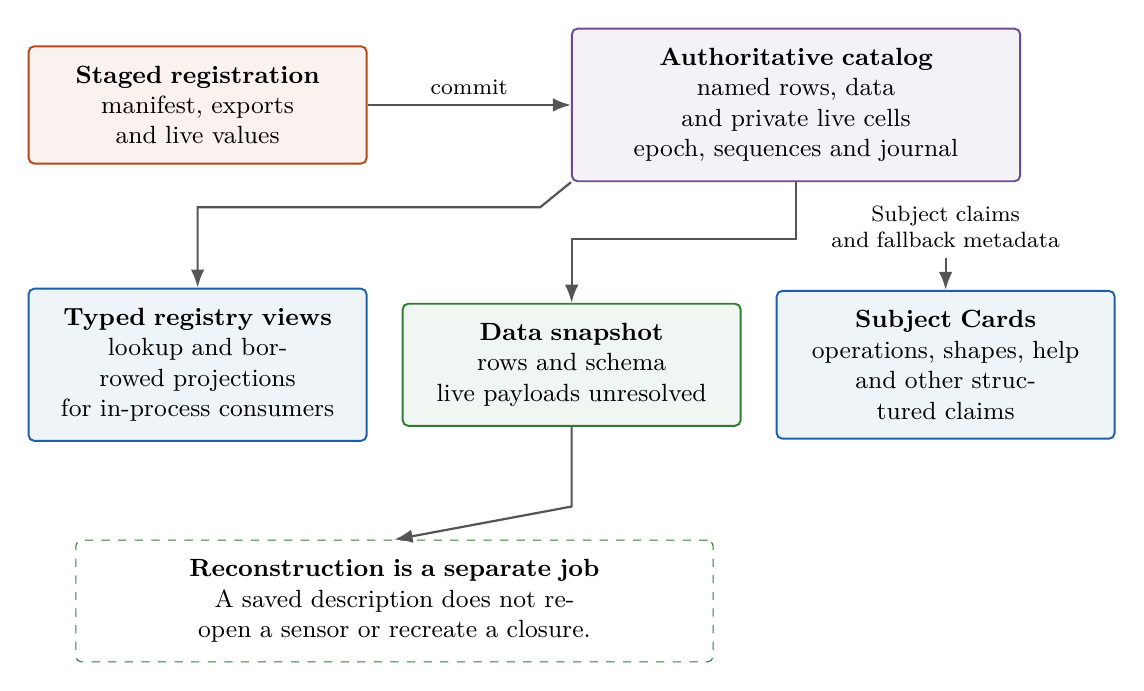
\begin{tikzpicture}[font=\small,
box/.style={draw=#1,fill=#1!7,rounded corners=2pt,line width=.7pt,text width=3.8cm,minimum height=1.45cm,align=center,inner sep=7pt},
arrow/.style={-{Latex[length=2.3mm]},line width=.8pt,draw=frameline}]
\node[box=elemB] (registration) at (-4.7,3.3) {\textbf{Staged registration}\\manifest, exports\\and live values};
\node[box=elemD,text width=5.2cm] (catalog) at (2.9,3.3) {\textbf{Authoritative catalog}\\named rows, data and private live cells\\epoch, sequences and journal};
\draw[arrow] (registration)--node[above,font=\footnotesize]{commit}(catalog);
\node[box=elemA] (lookup) at (-4.7,0) {\textbf{Typed registry views}\\lookup and borrowed projections\\for in-process consumers};
\node[box=elemC] (snapshot) at (.05,0) {\textbf{Data snapshot}\\rows and schema\\live payloads unresolved};
\node[box=elemA] (card) at (4.8,0) {\textbf{Subject Cards}\\operations, shapes, help\\and other structured claims};
\draw[arrow] (catalog.south west) -- (-.35,2) -- (-4.7,2) -- (lookup.north);
\draw[arrow] (catalog.south) -- (2.9,1.6) -- (.05,1.6) -- (snapshot.north);
\node[font=\footnotesize,align=center,text width=3.6cm] (claims) at (4.8,1.75)
 {Subject claims\\and fallback metadata};
\draw[arrow] (claims.south)--(card.north);

\node[draw=elemC,dashed,rounded corners=2pt,align=center,text width=7.6cm,inner sep=7pt] (restore) at (-2.2,-3)
 {\textbf{Reconstruction is a separate job}\\A saved description does not reopen a sensor or recreate a closure.};
\draw[arrow] (snapshot.south)--(.05,-1.8)--(restore.north);
\end{tikzpicture}
\end{document}
